% tesesusp.cls, v-0.0.1

% Based on 'bntex2ppgsi.cls', 'abntex2.csl' and on USP guidelines to create
% thesis and dissertation documents.
% See <https://www.overleaf.com/project/64f7bdf1641ad4a3a8482800>
% and <https://teses.usp.br/index.php?option=com_content&
%      view=article&id=52&Itemid=67&lang=en>
% to learn more.

\clearpage

% ----------------------------------------------------------------------
% Cover (mandatory)
% ----------------------------------------------------------------------

\imprimircapa

% ----------------------------------------------------------------------
% Title page (mandatory)
% ----------------------------------------------------------------------

%% Do not use this page for qualification exams.

\imprimirfolhaderosto*

% ----------------------------------------------------------------------
% Cataloging record (mandatory)
% ----------------------------------------------------------------------

%% Do not use for qualification exams.
\begin{fichacatalografica}
 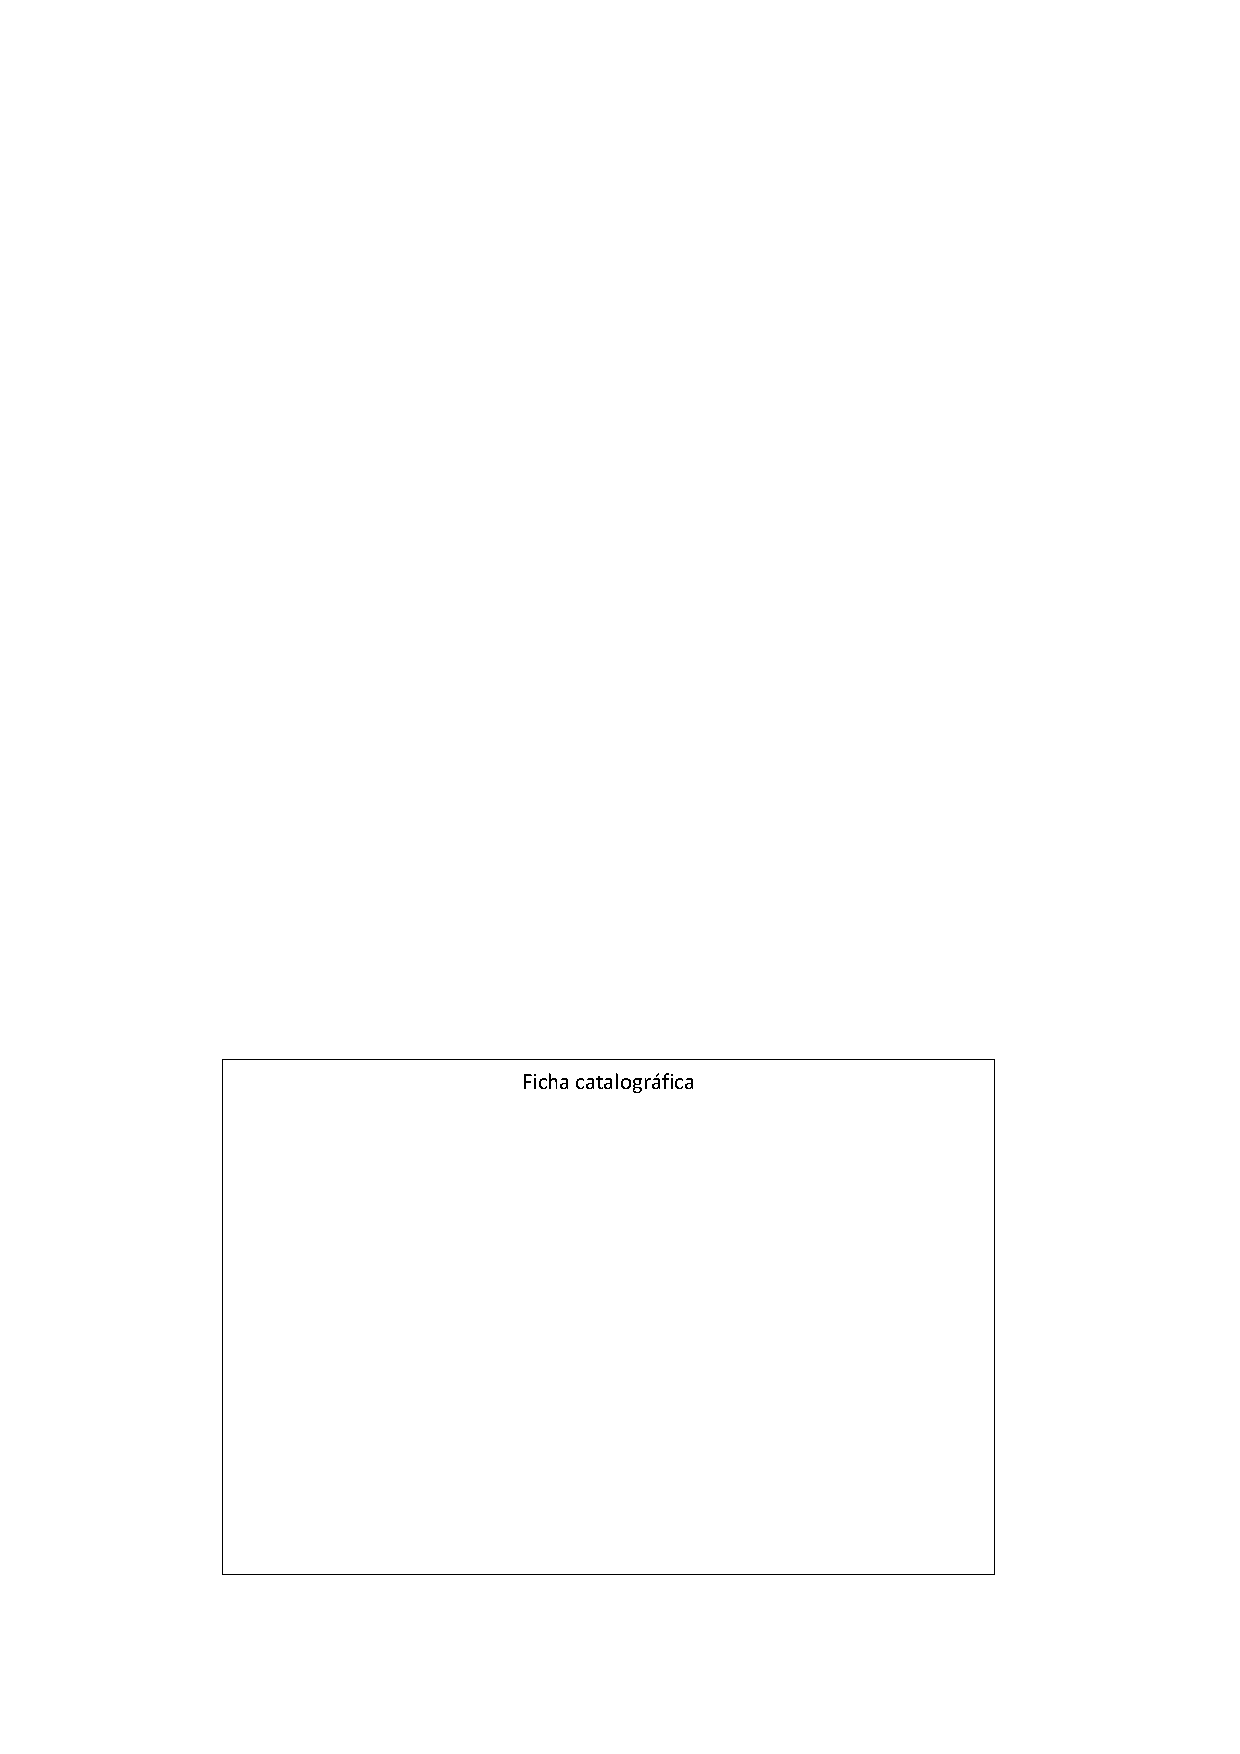
\includepdf{images/fig_ficha_catalografica.pdf}
\end{fichacatalografica}

% ----------------------------------------------------------------------
% Errata (optional)
% ----------------------------------------------------------------------

\begin{errata}
  \noindent
  This is the development version (<1.0.0) of this thesis. If needed, corrections will be listed here after its approval.
\end{errata}

% ----------------------------------------------------------------------
% Approval sheet (mandatory)
% ----------------------------------------------------------------------

\begin{folhadeaprovacao}
\noindent
Qualifying exam text by Daniel Vartanian, under the title \textbf{``\imprimirtitulo''}, presented to the School of Arts, Sciences, and Humanities at the University of São Paulo, as part of the requirements for the degree of Master of Science by the Graduate Program in Modeling Complex Systems (PPG-SCX), in the concentration area of Fundamentals of Complex Systems.

% Dissertation by Daniel Vartanian, under the title \textbf{``\imprimirtitulo''}, presented to the School of Arts, Sciences, and Humanities at the University of São Paulo, as part of the requirements for the degree of Master of Science by the Graduate Program in Modeling Complex Systems (PPG-SCX), in the concentration area of Fundamentals of Complex Systems.

\vspace*{1.5cm}

\noindent
Approved on: \_\_\_\_\_\_\_\_\_\_\_\_\_\_\_\_\_\_\_\_ , \_\_\_\_\_\_\_\_\_\_ .

\vspace*{1.5cm}

\begin{center}
Examination committee
\end{center}

\vspace*{0.5cm}

\renewcommand{\arraystretch}{2}
\noindent
\begin{tabular}{m{2cm} P{14cm}}
  Prof. Dr. & \_\_\_\_\_\_\_\_\_\_\_\_\_\_\_\_\_\_\_\_\_\_\_\_\_\_\_\_\_\_\_\_\_\_\_\_\_\_\_\_\_\_\_\_\_\_\_\_\_\_\_\_\_\_\_ \\
  Institution & \_\_\_\_\_\_\_\_\_\_\_\_\_\_\_\_\_\_\_\_\_\_\_\_\_\_\_\_\_\_\_\_\_\_\_\_\_\_\_\_\_\_\_\_\_\_\_\_\_\_\_\_\_\_\_ \\
  Evaluation & \_\_\_\_\_\_\_\_\_\_\_\_\_\_\_\_\_\_\_\_\_\_\_\_\_\_\_\_\_\_\_\_\_\_\_\_\_\_\_\_\_\_\_\_\_\_\_\_\_\_\_\_\_\_\_ \\
\end{tabular}

\vspace*{1cm}

\noindent
\begin{tabular}{m{2cm} P{14cm}}
  Prof. Dr. & \_\_\_\_\_\_\_\_\_\_\_\_\_\_\_\_\_\_\_\_\_\_\_\_\_\_\_\_\_\_\_\_\_\_\_\_\_\_\_\_\_\_\_\_\_\_\_\_\_\_\_\_\_\_\_ \\
  Institution & \_\_\_\_\_\_\_\_\_\_\_\_\_\_\_\_\_\_\_\_\_\_\_\_\_\_\_\_\_\_\_\_\_\_\_\_\_\_\_\_\_\_\_\_\_\_\_\_\_\_\_\_\_\_\_ \\
  Evaluation & \_\_\_\_\_\_\_\_\_\_\_\_\_\_\_\_\_\_\_\_\_\_\_\_\_\_\_\_\_\_\_\_\_\_\_\_\_\_\_\_\_\_\_\_\_\_\_\_\_\_\_\_\_\_\_ \\
\end{tabular}

\vspace*{1cm}

\noindent
\begin{tabular}{m{2cm} P{14cm}}
  Prof. Dr. & \_\_\_\_\_\_\_\_\_\_\_\_\_\_\_\_\_\_\_\_\_\_\_\_\_\_\_\_\_\_\_\_\_\_\_\_\_\_\_\_\_\_\_\_\_\_\_\_\_\_\_\_\_\_\_ \\
  Institution & \_\_\_\_\_\_\_\_\_\_\_\_\_\_\_\_\_\_\_\_\_\_\_\_\_\_\_\_\_\_\_\_\_\_\_\_\_\_\_\_\_\_\_\_\_\_\_\_\_\_\_\_\_\_\_ \\
  Evaluation & \_\_\_\_\_\_\_\_\_\_\_\_\_\_\_\_\_\_\_\_\_\_\_\_\_\_\_\_\_\_\_\_\_\_\_\_\_\_\_\_\_\_\_\_\_\_\_\_\_\_\_\_\_\_\_ \\
\end{tabular}
\end{folhadeaprovacao}

% ----------------------------------------------------------------------
% Inscription (optional)
% ----------------------------------------------------------------------

\begin{dedicatoria}
  \vspace*{\fill}
  \centering
  \noindent
  \textit{
  I dedicate this work to the skeptics, the radicals, the ignorant, the uncivilized, the subversives, the wild dogs, the irreducibles, the irreconcilables. To the true engines of change. To the destabilizers, who possess equal or greater importance than the stabilizers. To those who act on principle, even knowing that there is no ultimate reward or any meaning in life.
  }
	\vspace*{\fill}
\end{dedicatoria}

% ----------------------------------------------------------------------
% Acknowledgments (optional)
% ----------------------------------------------------------------------

\begin{agradecimentos}
  \noindent
  I would like to acknowledge this awesome \href{https://github.com/danielvartan/tesesusp}{Quarto format template}! :)
\end{agradecimentos}

% ----------------------------------------------------------------------
% Epigraph (optional)
% ----------------------------------------------------------------------

%% @theroyalsociety

\begin{epigrafe}
  \vspace*{\fill}
	\begin{flushright}
	  \textit{Nullius in verba} \\
		(The Royal Society, n.d.)
	\end{flushright}
\end{epigrafe}

% ----------------------------------------------------------------------
% Abstract in the vernacular language (mandatory)
% ----------------------------------------------------------------------

\setlength{\absparsep}{18pt}
\begin{resumo}

\begin{flushleft}
[Surname], [Initials]. ([Year]). \textit{[Title]} [(Master's/PhD) thesis]. [Department/School], [University], [City]. [URL]
\end{flushleft}

Lorem ipsum dolor sit amet, consectetur adipiscing elit. Pellentesque accumsan rutrum lacus, vitae iaculis nisi bibendum in. Nulla et pellentesque nisl. Proin mollis dui sit amet egestas fermentum. Maecenas eu odio odio. Aenean porta ipsum in mauris pharetra dapibus. Nunc dapibus libero nec dui lacinia, id ultricies lectus maximus. Mauris quis mauris in velit pulvinar rutrum. Cras congue ante in orci luctus placerat. Nullam sit amet nisi augue. Maecenas non ligula eros. Etiam nec dolor a mi bibendum auctor.

Keywords: Keyword 1. Keyword 2. Keyword 3.
\end{resumo}

% ----------------------------------------------------------------------
% Abstract in the foreign language (mandatory)
% ----------------------------------------------------------------------

\begin{resumo}[RESUMO]
\begin{otherlanguage*}{brazil}

\begin{flushleft}
[Sobrenome], [Iniciais]. ([Ano]). \textit{[Título]} [(Tese/Dissertação) de (Mestrado/Doutorado)]. [Departament/Escola], [Universidade], [Cidade]. [URL]
\end{flushleft}

Lorem ipsum dolor sit amet, consectetur adipiscing elit. Pellentesque accumsan rutrum lacus, vitae iaculis nisi bibendum in. Nulla et pellentesque nisl. Proin mollis dui sit amet egestas fermentum. Maecenas eu odio odio. Aenean porta ipsum in mauris pharetra dapibus. Nunc dapibus libero nec dui lacinia, id ultricies lectus maximus. Mauris quis mauris in velit pulvinar rutrum. Cras congue ante in orci luctus placerat. Nullam sit amet nisi augue. Maecenas non ligula eros. Etiam nec dolor a mi bibendum auctor.

Palavras-chaves: Palavra-chave 1. Palavra-chave 2. Palavra-chave 3.
\end{otherlanguage*}
\end{resumo}

% ----------------------------------------------------------------------
% List of figures (optional)
% ----------------------------------------------------------------------

\renewcommand{\listfigurename}{LIST OF FIGURES}
\pdfbookmark[0]{\listfigurename}{lof}
\listoffigures*
\cleardoublepage

% ----------------------------------------------------------------------
% List of tables (optional)
% ----------------------------------------------------------------------

\renewcommand{\listtablename}{LIST OF TABLES}
\pdfbookmark[0]{\listtablename}{lot}
\listoftables*
\cleardoublepage

% ----------------------------------------------------------------------
% List of abbreviations and acronyms (optional)
% ----------------------------------------------------------------------

\begin{siglas}
  \item[Abbreviation 1] Abbreviation expanded definition
  \item[Abbreviation 2] Abbreviation expanded definition
  \item[Abbreviation 3] Abbreviation expanded definition
  \item[Abbreviation 4] Abbreviation expanded definition
  \item[Abbreviation 5] Abbreviation expanded definition
  \item[Abbreviation 6] Abbreviation expanded definition
  \item[Abbreviation 7] Abbreviation expanded definition
  \item[Abbreviation 8] Abbreviation expanded definition
  \item[Abbreviation 9] Abbreviation expanded definition
  \item[Abbreviation 10] Abbreviation expanded definition
\end{siglas}

% ----------------------------------------------------------------------
% List of symbols (optional)
% ----------------------------------------------------------------------

\begin{simbolos}
  \item[$\Gamma$] Gamma
  \item[$\Lambda$] Lambda
  \item[$\zeta$] zeta
  \item[$\in$] In/Belongs
\end{simbolos}

% ----------------------------------------------------------------------
% Table of contents (mandatory)
% ----------------------------------------------------------------------

\renewcommand{\contentsname}{TABLE OF CONTENTS}
\pdfbookmark[0]{\contentsname}{toc}
% \tableofcontents*
\cleardoublepage
